\section{Previous Research}
\label{Previous_Research}
This section summarizes four important papers, which all made a big impact in the area of deep reinforcement learning. The most important concepts are described for each of the papers. The section will give an overview of the state-of-the-art in deep reinforcement learning.    

\subsection{Playing Atari with Deep Reinforcement Learning }
The paper \cite{DBLP:journals/corr/MnihKSGAWR13} was published in 2013 by DeepMind Technologies. It is the first paper to make a deep learning model to successfully learn control policies directly from sensory input using reinforcement learning. 

The paper presents some of the challenges by using deep learning to do reinforcement learning. One of the challenges is that the deep learning algorithms require a large amount of hand-labeled training data. Another challenge is the delay between action and resulting reward, which can be thousands of time-steps long. The paper demonstrates that a convolutional neural network can overcome these challenges.  

The paper's goal is to connect a reinforcement learning algorithm to a deep neural network which uses RGB images and processes training data by using stochastic gradient updates. The starting point for this approach is to use Tesauro's TD-Gammon \cite{Tesauro:1995:TDL:203330.203343} architecture. The network is different from TD-Gammon and other online approaches because it uses a technique known as experience replay, where the agent stores it's own experiences at each time-step.

The input to the neural network is an $84 \times 84 \times 4$ image. The output from the neural network is a value for each valid action. The architecture of the network can be seen on \Cref{fig:playing_atari}.
   
\begin{figure}[H]
	\centering
	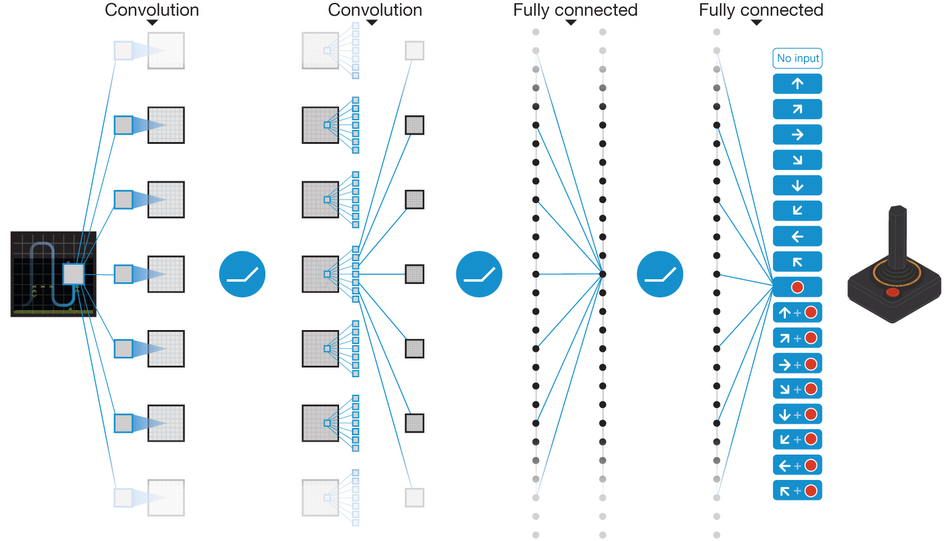
\includegraphics[width=0.825\textwidth]{Figures/TheoreticalBackground/playing_atari.jpg}
	\caption{The architecture of the network used in the article "Playing Atari with Deep Reinforcement Learning" \cite{DBLP:journals/corr/MnihKSGAWR13}}
	\label{fig:playing_atari}
\end{figure} 

This network is tested on seven Atari games, and the approach in this paper gave the state-of-the-art result in six of the seven games. Finally, it showed better performance than an expert human player in three out of the seven games. The Deep Q-Network method used in the paper is explained thoroughly in \Cref{sec:DQN}.

\subsection{Mastering the Game of Go with Deep Neural Networks and Tree Search}
The paper \cite{Silver_2016} introduces a new approach for competing in the classic game of Go \cite{explain_go}. The paper was published in 2016. The game of Go is the most challenging classic game for artificial intelligence, due to the enormous search space and the difficulty of evaluating board positions and moves.

The structure of the implementation employs a similar architecture as in \cite{DBLP:journals/corr/MnihKSGAWR13}. The board position is passed in as a $19 \times 19$ image and convolutional layers are used to construct a representation of the position. Neural networks are used to reduce the search space by making use of the value networks to evaluate board position and policy networks to select moves.

The way the Neural Network was trained started with training a supervised learning policy network, directly from expert human moves. Next training is the reinforcement learning policy network. This policy improves the supervised learning network and optimizes the outcome of the played games with self-play. The final step of training is to train the value network, that predicts the winner of the game played by the reinforcement learning policy network against itself. 

By combining tree search with policy and value networks, \textit{AlphaGo} has reached a professional level in Go. In March 2016 \textit{AlphaGo} won with the score 4-1 against the legendary Lee Sedol, the top Go player in the world over the past decade.

\subsection{Asynchronous Methods for Deep Reinforcement Learning}\label{AsyncMeths}
This is another paper \cite{DBLP:journals/corr/MnihBMGLHSK16} from the team behind \cite{DBLP:journals/corr/MnihKSGAWR13} paper, and was published in 2016. This paper provides a very different paradigm for deep reinforcement learning. Instead of experience replay, it asynchronously executes multiple agents in parallel, on multiple instances of the environment. 

This simple idea enables a much larger spectrum of the on-policy as well as off-policy reinforcement learning algorithms, to be applied robustly and effectively using deep neural networks. It also offers practical benefits - this experiment can run on a single machine with a standard multi-core CPU, instead of GPUs.

The paper presents asynchronous versions of four standard reinforcement algorithms used on different platforms. The platform used is a simulator for Atari 2600, Torcs 3D car racing simulator, Mujoco, and Labyrinth. The asynchronous advantage actor-critic (A3C) algorithm resulted in the best performing agent on all the platforms.

The A3C beats the state-of-the-art result in 26 of 57 Atari games. This is a big improvement from previous reinforcement networks. When trained on the Atari domain using 16 CPU cores, the proposed asynchronous algorithm trains faster than the Deep Q-Network trains on a Nvidia K40 GPU, with A3C surpassing the state-of-the-art with half the training time. The A3C method is explained more in details in \Cref{sec:A3C}.
   
\subsection{Deep Reinforcement Learning framework for Autonomous Driving} 
The paper \cite{Sallab:2017:2470-1173:70} is motivated by the papers \cite{DBLP:journals/corr/MnihKSGAWR13} and \cite{Silver_2016}. It proposes a framework for autonomous driving using deep reinforcement learning. The paper was published in 2017. It is relevant because it is difficult to handle autonomous driving as a supervised learning problem due to interactions with the environment. It also integrates recent work on attention models, to focus on relevant information, thereby reducing the computational complexity.

They propose a framework for an end-to-end autonomous driving model that takes in raw sensor input and outputs the driving actions. The model can handle partially observable scenarios.  

The framework can be seen on \Cref{fig:Framework_article}. In the model, the spatial features are extracted via a CNN, which learns the features from data. In order to decode the true environment state, an LSTM network is used, which can control what information to keep from previous the state. The final part of the framework is the reinforcement planning part. The inputs are the states of the environment and their aggregations over time. The output of the framework are the driving actions.  

The paper used The Open-source Racing Car Simulator (TORCS) with a lane keeping assist algorithm to test the framework. The result is a successful lane keeping behavior with the speed limit.       

\begin{figure}[H]
	\centering
	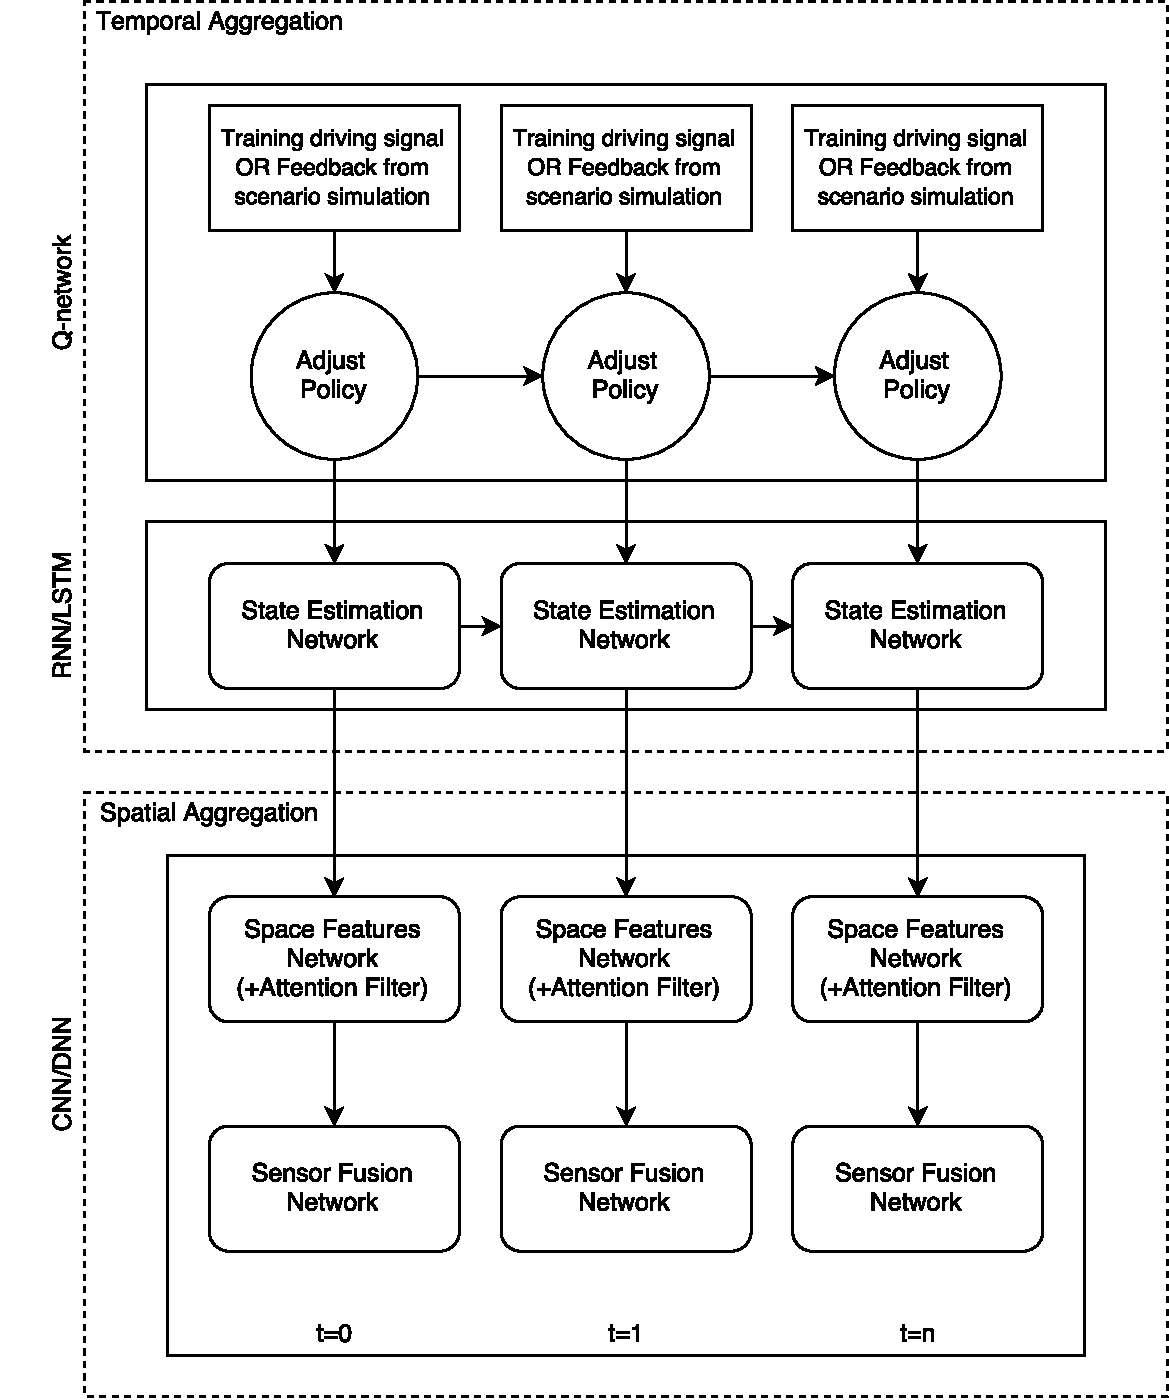
\includegraphics[width=0.8\textwidth]{Figures/TheoreticalBackground/Framework_article}
	\caption{Framework from the article "Deep Reinforcement Learning framework for Autonomous Driving" \cite{Sallab:2017:2470-1173:70} }
	\label{fig:Framework_article}
\end{figure}
 
This concludes the theoretical background chapter. The chapter presented the problem of reinforcement learning with its mathematical models and the known basic solution methods. Also, a couple of state-of-the-art articles were summarized here. The next chapter presents the approaches of solving a real-world problem, the problem of driver-less cars more precisely, with some of the advanced RL methods.